\documentclass[11pt]{article}

%%%%%%%%%%%%%%%%%%
% Basic packages %
%%%%%%%%%%%%%%%%%%

\usepackage[T1]{fontenc}
\usepackage[utf8]{inputenc}
\usepackage[british]{babel}
\usepackage[stretch = 25, shrink = 25, tracking=true, letterspace=30]{microtype}

\usepackage{geometry}
 \geometry{
 a4paper,
 %total={150mm,257mm},
 left=25mm,
 right=25mm,
 top=15mm,
 } % Page Layout
\usepackage[dvipsnames]{xcolor} % Colour
\usepackage{amsmath} % Maths

%%%%%%%%%%%%%%%%%%%
% Tables, figures %
%%%%%%%%%%%%%%%%%%%

\usepackage{float}
\usepackage{graphicx} % Imgages, figures
\graphicspath{{./figures/}} % Set figure path

\usepackage{booktabs} % Pretty tables

%%%%%%%%%%%%%
% Citations %
%%%%%%%%%%%%%

\usepackage[
    backend=biber,
    style=apa,
    sortlocale=de_DE,
    natbib=true,
    url=false, 
    doi=true,
    eprint=false
]{biblatex}

%\addbibresource{ASSIGNMENT_1.bib} %Imports bibliography file
\usepackage{csquotes} % used for block quotes

%%%%%%%%%
% Fonts %
%%%%%%%%%

%%% Helvetica:
%\usepackage[scaled=0.95]{helvet} % Imports Helvetica, which is similar to Arial
%\renewcommand{\rmdefault}{phv} % Use Helvetica

%%% Atkinson Hyperlegible, nerdy font 
%\usepackage[sfdefault]{atkinson} %% Option 'sfdefault' if the base
%% font of the document is to be sans serif.
%\usepackage[T1]{fontenc}

%%%%%%%%%%%%%%%%%%
% Header setting %
%%%%%%%%%%%%%%%%%%

\usepackage{titlesec} % pretty headers
\titleformat{\section}
  {\normalfont\large\bfseries\color{Black}} % Formatting options
  {\thesection}{1em}{}

%%%%%%%%%%%%%%%%%%
% Title settings %
%%%%%%%%%%%%%%%%%%

\title{\textcolor{Plum}{\textbf{COMP527 - CA Assignment 2 - Preprocessing}}}
\author{\textbf{Pablo Ramos - 201885602}}

\setlength\parindent{10mm}

%%%%%%%%%%%%
%%% BODY %%%
%%%%%%%%%%%%

\begin{document}
% Dark Mode - Comment the bottom 2 lines to get a normal white page
%\pagecolor{black}
%\color{white} % Set the default colour to white
%
%\pagenumbering{gobble} % Turns off page numbering
%
\maketitle
{\setlength{\parindent}{0mm}{\color{Plum} \rule{\linewidth}{0.5mm}}} % Lines with colour options

\section{Overview of the Pipeline}

\texttt{clustering.py} loads and cleans the data, generates sentence embeddings using SBERT, reduces dimensionality with UMAP, and then applies K-Means with silhouette analysis to determine the optimal number of clusters.

\section{Sentence-BERT (SBERT)}

BERT is a kind of sentence transformer. It takes text as input and transforms it into fixed-length vector representations. These vectors are treated as tensors carrying the semantic meaning of the text, and BERT, being a compact language model, can easily obtain abstractions from the data snippets. SBERT was build on top of BERT to also be computationally efficient retrieve better information from various sentences.

\texttt{all-MiniLM-L6-v2} is a pretrained SBERT readily implemented with the python library sentence transformers. It runs locally and is adequate for short sentence clustering.

\section{UMAP}

Because the vectors outputted by SBERT have a long length, and thus live on a very high dimensional space, for clustering to work properly it's necessary to map the vectors onto a lower dimensional space. To do that, UMAP was implemented.

One of UMAP's hyperparameters is n components. Increasing it reduces the strength of a single unique cluster and prioritises global grouping. Different values were tested (10, 20, 30 and 40), with 40 being the optimal one. A function to print the headers of the clusters on the best K was implemented. This allowed manually reading the results, and see if the clusters actually made any sense.

\section{K-Means Clustering}
K means is a clustering algorithm that can be trained without any labels on the data. Because the given dataset has raw text sentences with no additional context, this method is adequate for the clustering.

K means will try to cluster the data in an increasing number of clusters (K) and will then measure how well the chosen centroids contain each cluster. For every K, a k number of centroids if randomly placed on the map, and the average distance of the data points in that centroids region is calculated. The position is then progressively adjusted to optimise for the lowest possible average distance of every cluster's data point to its centroid.

\section{Silhouette Analysis}

Silhouette analysis was used to determine the optimal number of clusters $K$. For each data point, the silhouette coefficient $s$ is defined as:

\begin{center}
  $s = \frac{b - a}{\max(a, b)}$
\end{center}

{\setlength{\parindent}{0mm}where $a$ is the mean intra-cluster distance and $b$ is the mean distance to the nearest neighbouring cluster. Values range from $-1$ (poor) to $1$ (ideal). $K=1$ is hardcoded to a score of 0 as the coefficient is undefined for a single cluster.}

\begin{figure}[H]
  \centering
  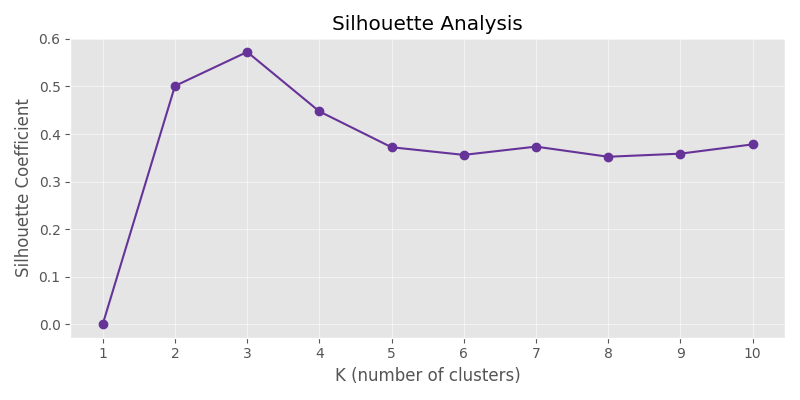
\includegraphics[width=0.8\textwidth]{sberf_silhouette_plot.png}
  \caption{Silhouette coefficients for $K = 1$ to $10$.}
  \label{fig:silhouette}
\end{figure}

\section{Optimal $K$ and Results}

The best K was 3. The major groups can be described as Coriolanus, American slice of life, and Academic slice of life. This largely makes sense, and for k=3 the silhouette coefficient is 0.5727. Given that a good value is considered to be 0.5, this can be treated as a good result.

The cluster here described as Academic slice of life had a strong semantic signal (I.E. very distant vectors), and thus it had its own cluster and everything else was randomly grouped together. The only tuning required to fix this was optimising UMAP as previously stated.

%\printbibliography

\end{document}